\chapter{Project Analysis}\label{ch:project-analysis}

\section{Stakeholder Analysis}\label{sec:stakeholders-analysis}
Developing a platform like Chronocademy required a strong awareness of the various stakeholders involved.\ Recognizing and categorizing these stakeholders provided the team with a clearer understanding of the platform’s purpose, requirements hierarchy, and potential challenges.\ By addressing these three core aspects, the team ensured a professional and structured approach to project development.

For clarity, we define a stakeholder as:

\begin{quote}
``A person or group of people who own a share in a business or a person such as an employee, customer, or citizen who is involved with an organization, society, etc.\ and therefore has responsibilities towards it and an interest in its success.''
\end{quote}\cite{stakeholder}

In this section, the reader will find a list of all the potential stakeholders, should this business succeed:

\begin{itemize}
\item Learners (Primary Users): Individuals looking to acquire new skills but constrained by financial barriers.\ They are the primary audience, relying on the platform to find suitable courses and teachers.
\item Teachers (Primary Users): Individuals with expertise in specific skills who want to share their knowledge.\ They use the platform to offer lessons and earn time credits, motivating them to participate actively.
\item Platform Administrators (Internal Stakeholders): The team responsible for maintaining, managing, and improving the platform.\ They ensure smooth operations, manage user accounts, and resolve technical issues.
\item Developers (Internal Stakeholders): The technical team responsible for building, deploying, and maintaining the Chronocademy application.\ Their role is crucial for implementing features and ensuring performance and security.
\item Investors/Sponsors (External Stakeholders): Individuals or organizations that fund the platform’s development or support its long-term goals.\ Their interest lies in the platform’s growth, user base, and potential returns.
\item Educational Institutions (External Stakeholders): Schools, training centers, or non-profit organizations that might collaborate with the platform to offer courses or expand their reach.
\item Community Members (Indirect Stakeholders): Families, friends, or networks of users who may indirectly benefit from the platform by accessing shared skills or recommendations.
\item Hosting and Service Providers (External Stakeholders): Companies like Fly.io or other infrastructure providers that support the hosting, storage, and scalability of the platform.\ Their stability and reliability directly impact Chronocademy’s performance.
\item Regulatory Bodies (External Stakeholders): Authorities ensuring that the platform complies with local laws, including data protection, financial transactions, and online education standards.
\end{itemize}

\subsection{Stakeholder Identification}\label{subsec:stakeholders-identification}
After recognizing all the involved parties and categorizing them as stakeholders, a power-interest matrix was created to group them by their level of influence and interest.\ This tool helped us to understand how to address each group during our project development.

\subsubsection*{1. Manage Closely (High Influence, High Interest):}
\begin{itemize}
\item Investors/Sponsors: Fund the platform and influence its strategic direction.
\item Developers: Build and maintain the system; essential for success.
\end{itemize}

\subsubsection*{2. Keep Satisfied (High Influence, Low Interest):}
\begin{itemize}
\item Regulatory Bodies: Ensure compliance with laws and regulations; their approval is crucial but their active interest is low.
\item Hosting and Service Providers: Provide infrastructure reliability; influence platform uptime but have limited engagement with the project.
\end{itemize}

\subsubsection*{3. Keep Informed (Low Influence, High Interest):}
\begin{itemize}
\item Learners (Core Users): Highly engaged users eager to access educational resources.\ Their satisfaction and feedback shape the platform’s usability.
\item Teachers (Core Users): Key contributors interested in sharing their skills and engaging with the system.
\end{itemize}

\subsubsection*{4. Monitor (Low Influence, Low Interest):}
\begin{itemize}
\item Community Members: Indirectly impacted by the platform; limited influence and occasional involvement.
\end{itemize}

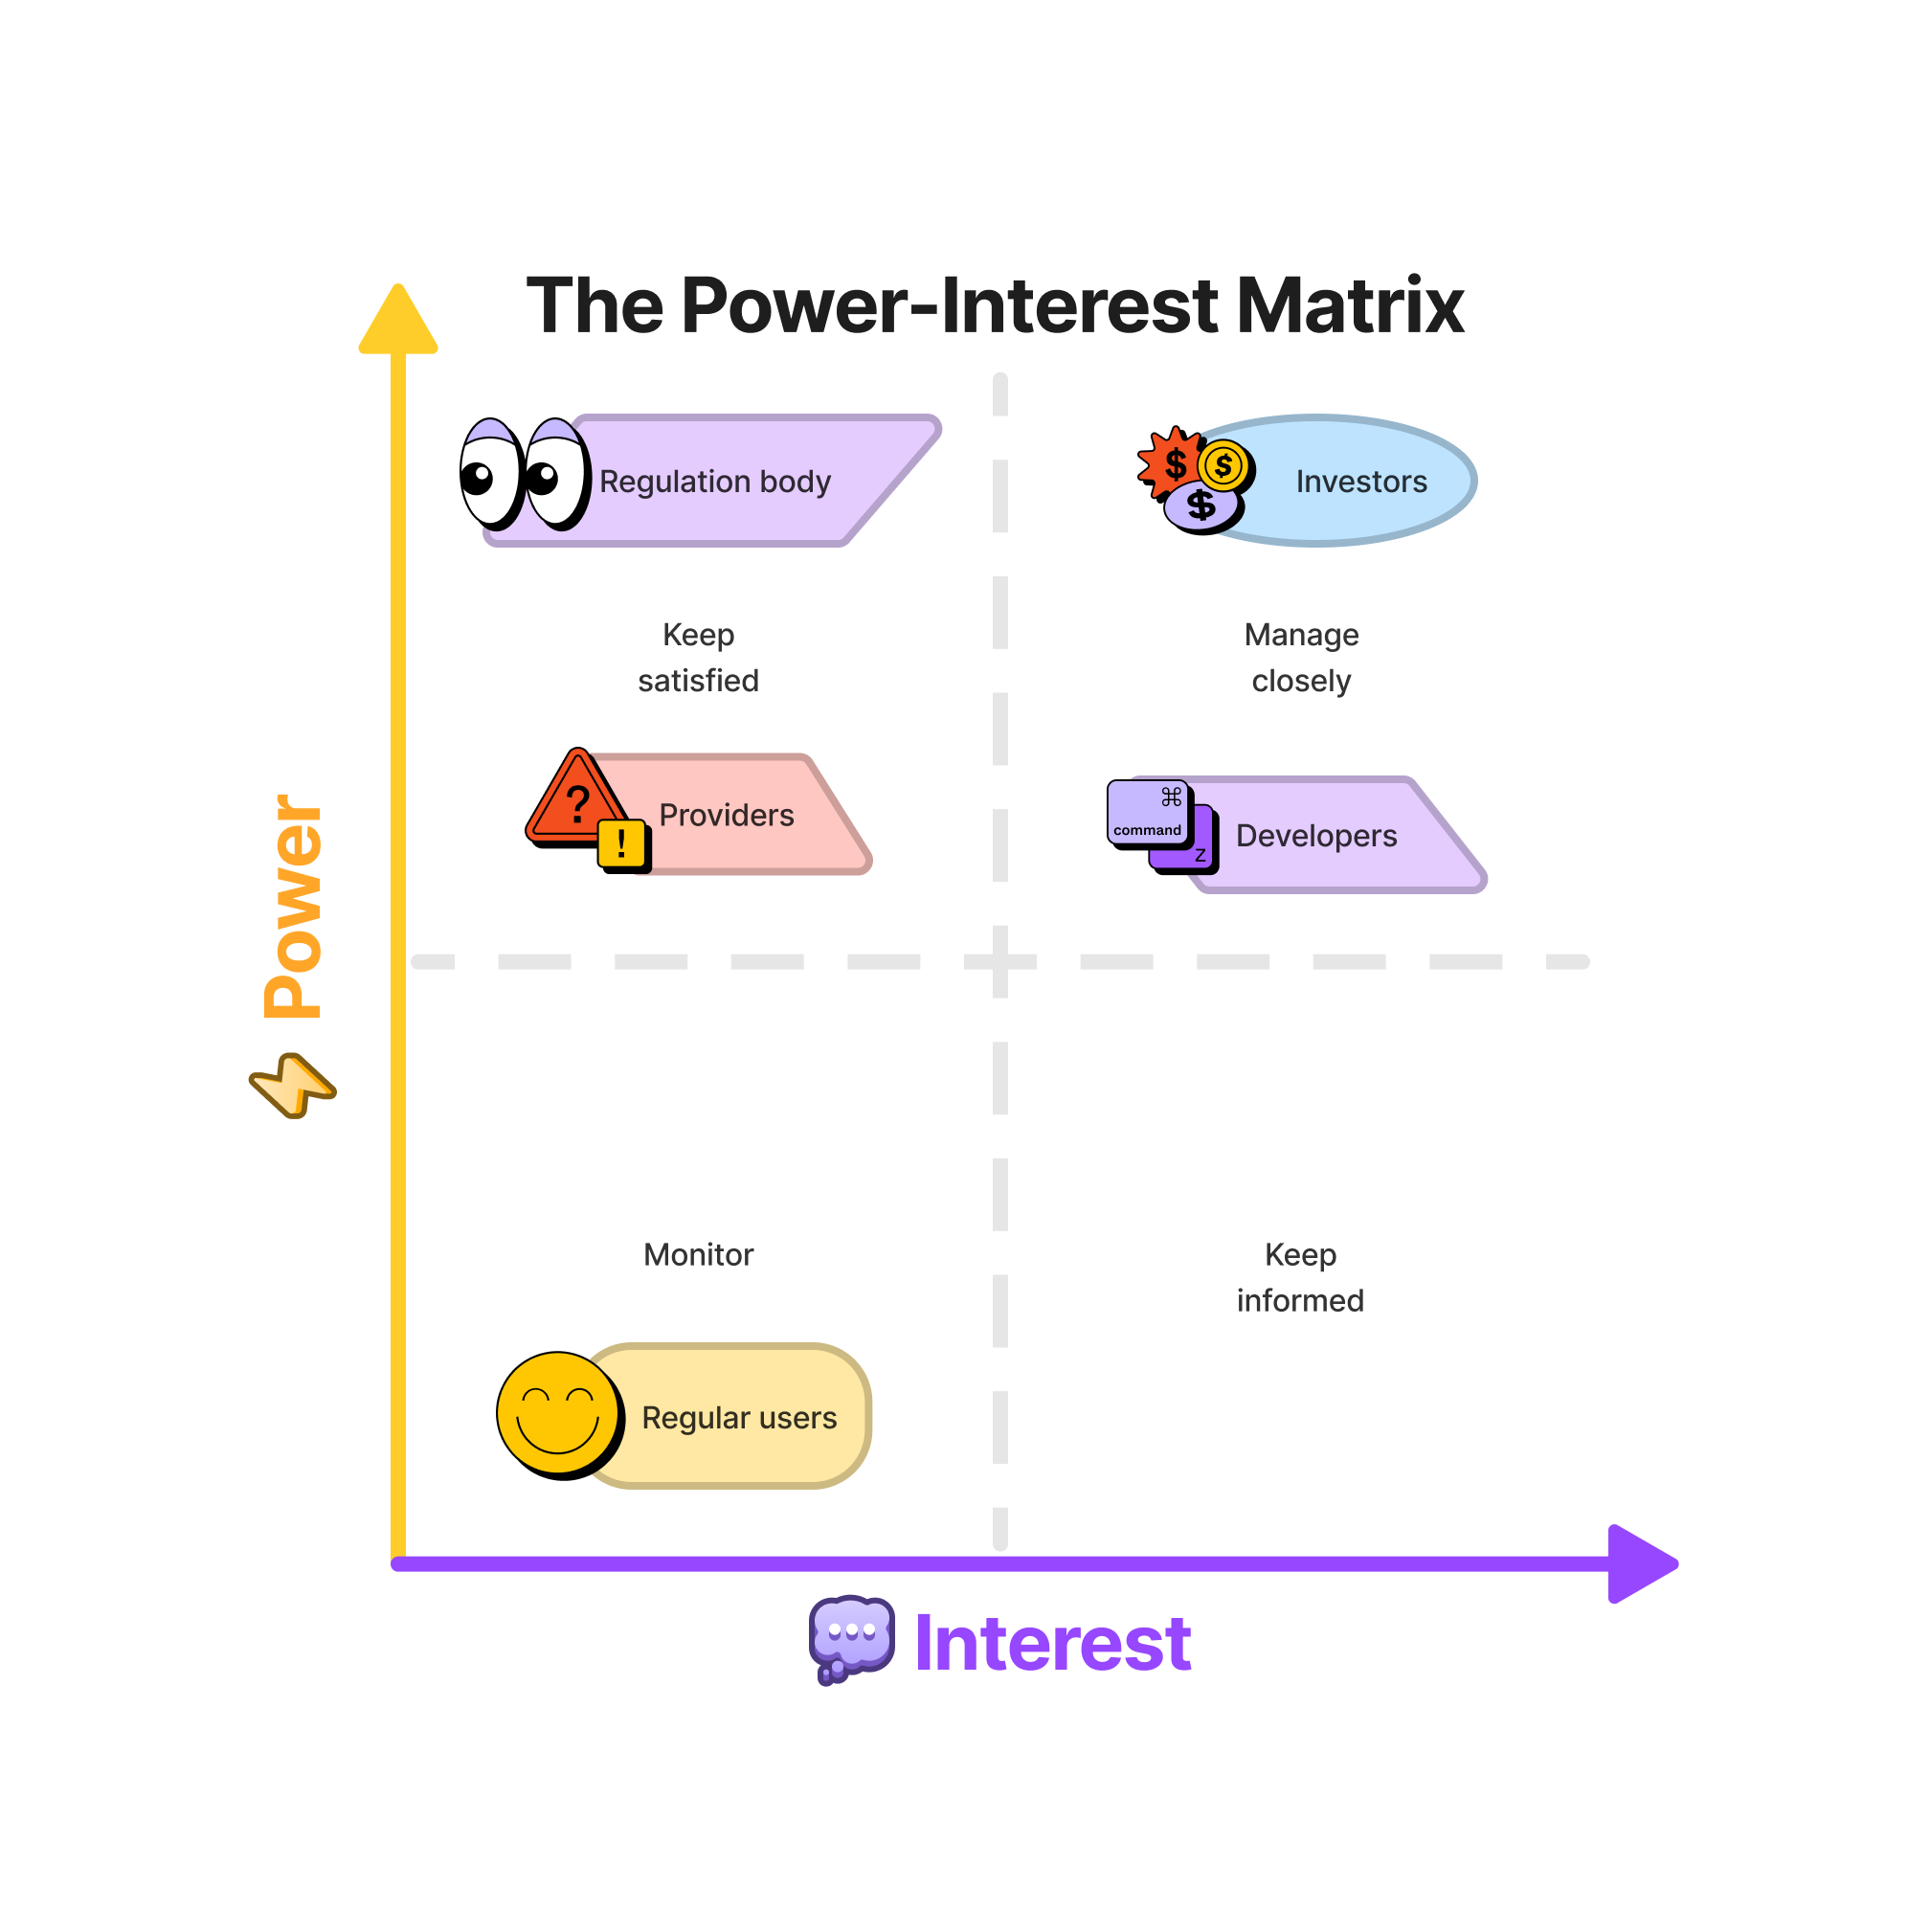
\includegraphics[width=400px]{stakeholder-matrix}